\section{Trace-driven Evaluation}
\label{sec:sim}

In this section we evaluate \dtrack{} with trace-driven simulations
using the data set described in \secstr~\ref{sec:char}.  We focus
on comparing the probing cost of remapping path changes using complete
versus local remapping.

\subsection{Probing cost}

Local remapping's probing cost varies according to the radius $r^\prime$
where \dtrack{} detected the change.  \figstr~\ref{fig:sim.rmprt.start}
shows the distribution of local remapping's probing cost for the
minimum, average, and maximum costs, calculated over all radii where
\dtrack{} can detect each change.  We see that the distributions of
minimum and maximum costs are similar.  Many path changes add or remove
few hops, so there are few radii where \dtrack{} can detect the path
change and little variation in probing cost.  In the rest of this
section, we use the average cost as local remapping's probing cost.

% \begin{figure}
% \begin{center}
% 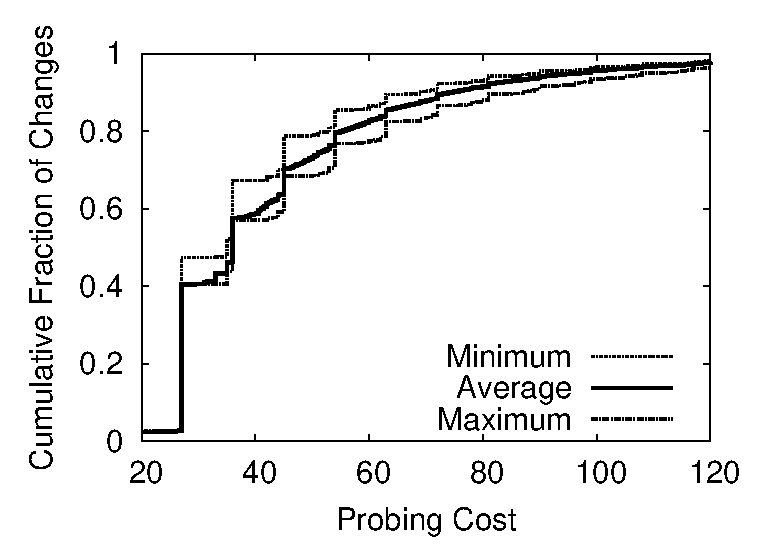
\includegraphics[width=0.8\columnwidth]{figs/rmprtcost.eps}
% \caption{\rmprt{}'s remapping cost varying the hop
% $\boldsymbol{h^\prime}$ where a change is detected.}
% \label{fig:sim.rmprt.start}
% \end{center}
% \end{figure}

\figstr~\ref{fig:sim.abs.cmp} compares probing costs for both local and
complete remapping.  Despite the binary search to locate local change
zones and the need to measure convergence and divergence hops, local
remapping reduces probing costs considerably compared to complete
remapping.  \figstr~\ref{fig:sim.abs.cmp.hops} compares the number of
hops measured by the two approaches.  Comparing with
\figstr~\ref{fig:char.nrouters}, we see that local remapping frequently
measures more hops than the number of added hops, but still only a small
fraction of all hops in a route, shown by the ``complete remapping''
curve.  Local remapping measures at least three hops for 99.6\% of path
changes, even though about 9\% of path changes in our data set only
remove hops from the path (\figstr~\ref{fig:char.nrouters}).  $\LCZ$s
that only remove hops are remapped by the binary search phase of our
algorithm, which takes at least three probes except when $r' < 4$ (which
happens in 0.4\% of path changes in our data).  The remap phase in our
algorithm also measures at least three hops to remap an $\LCZ$: $r_d$,
$r_c$, and changed hops in between.

% \begin{figure}
% \begin{center}
% 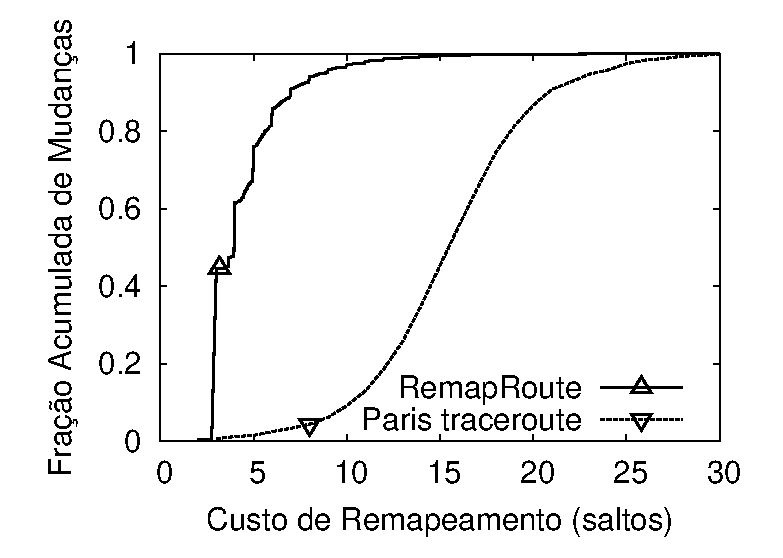
\includegraphics[width=0.8\columnwidth]{figs/costcmp.eps}
% \caption{Comparison of remapping cost between \rmprt{} and Paris
% traceroute.}
% \label{fig:sim.abs.cmp}
% \end{center}
% \end{figure}

\figstr~\ref{fig:sim.savings.cmp} shows the distribution of probing cost
savings when using local remapping instead of complete remapping.  We
compute probing cost savings as $(C_\mathrm{complete} -
C_\mathrm{local})/C_\mathrm{complete}$, where $C_\mathrm{complete}$ and
$C_\mathrm{local}$ are complete and local remapping's probing costs,
respectively.  The solid line, computed for all path changes in our data
set, shows that cost savings are significant.  Local remapping reduces
probing cost by more than half for 88\% of path changes, and reduces the
overall probing cost by 73\%.  The dashed lines in
\figstr~\ref{fig:sim.savings.cmp} show probing cost savings for routes
shorter than 10 hops (labelled ``short'') and routes longer than 20 hops
(labelled ``long'').  Local remapping probing cost savings is higher for
long routes, where complete remapping wastes probes in many hops that
have not changed.

% Local remapping reduces number of hops measured by more than half for
% 88\% of path changes.

\begin{figure}
\begin{center}
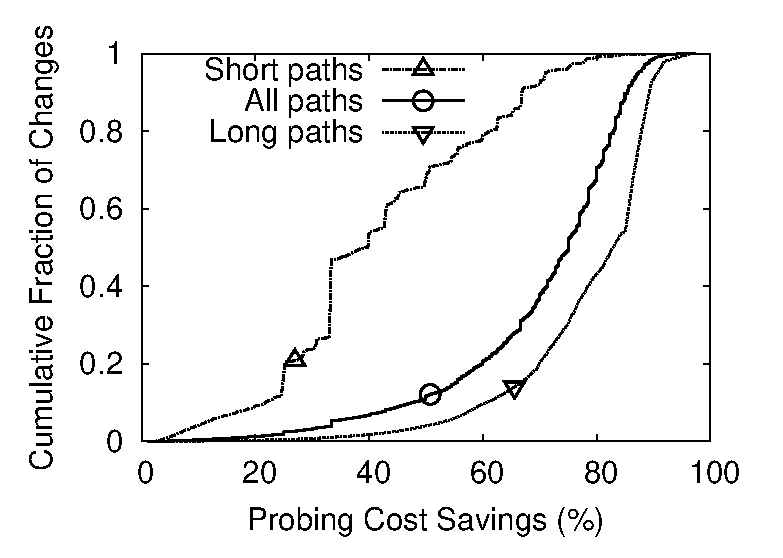
\includegraphics[width=0.8\columnwidth]{figs/probsavings.eps}
\caption{Probing cost savings of local remapping over complete
remapping.}
\label{fig:sim.savings.cmp}
\end{center}
\end{figure}

% FIGS. 9--11 FROM SEC. 6
\begin{figure*}
\vspace{5mm}
\begin{minipage}{0.33\textwidth}
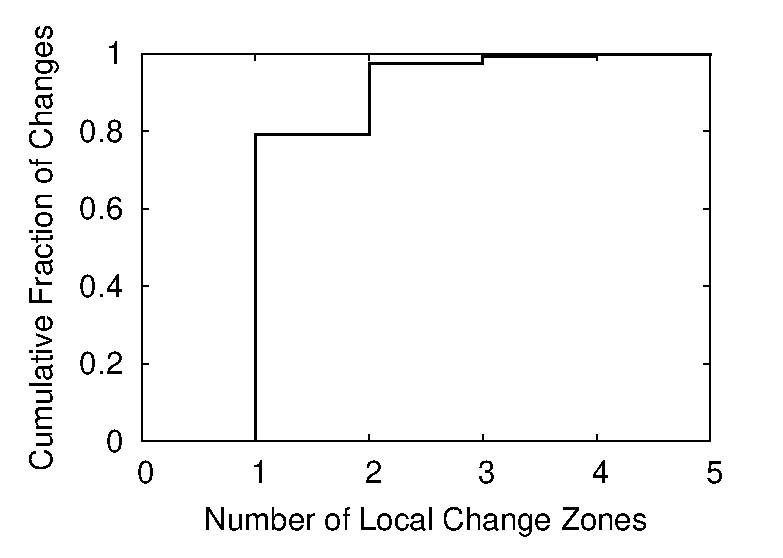
\includegraphics[width=1.05\textwidth]{figs/ndisjoint.eps}
\caption{Number of local change zones in path changes.}
\label{fig:sim.ndisjoint}
\end{minipage}
\hfill
\begin{minipage}{0.33\textwidth}
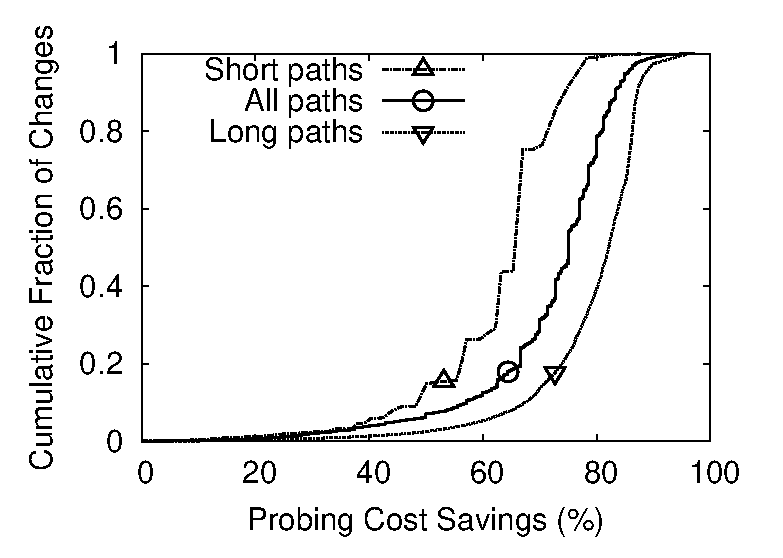
\includegraphics[width=1.05\textwidth]{figs/probsavingsreal.eps}
\caption{Probing cost savings with local remapping in a real
deployment.}
\label{fig:deploy.savings}
\end{minipage}
\begin{minipage}{0.33\textwidth}
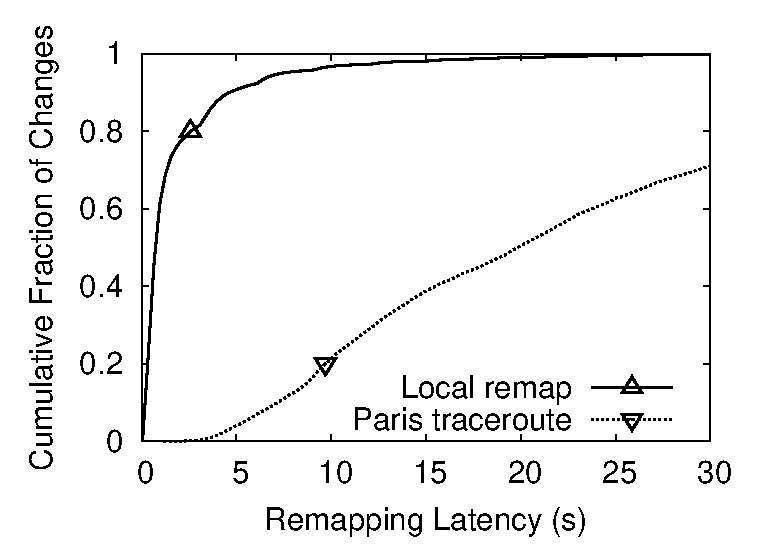
\includegraphics[width=1.05\textwidth]{figs/latencies.eps}
\caption{Comparing remap latency in the real deployment.}
\label{fig:deploy.latency}
\end{minipage}
\end{figure*}

\subsection{Remapping errors}
\label{sec:remap.errors}

Local remapping may only remap parts of a path change when it is
composed of multiple $\LCZ$s.  For example, a route
$p_{i-1} = [s, I_1, I_2, I_3, I_4, I_5, d]$ may change to $p_i =[s, I_1, I_6, I_3, I_9, I_5, d]$.  
In this case there are two local change zones at $(r_d,r_c)=(1,3)$ and $(r_d,r_c)=(3,5)$,
which  \dtrack{} could detect for example as $\LCZ(r'=2)$ or $\LCZ(r'=4)$. 
Local remapping could remap either depending on where the change was detected.

% \begin{minipage}{0.33\textwidth}
% 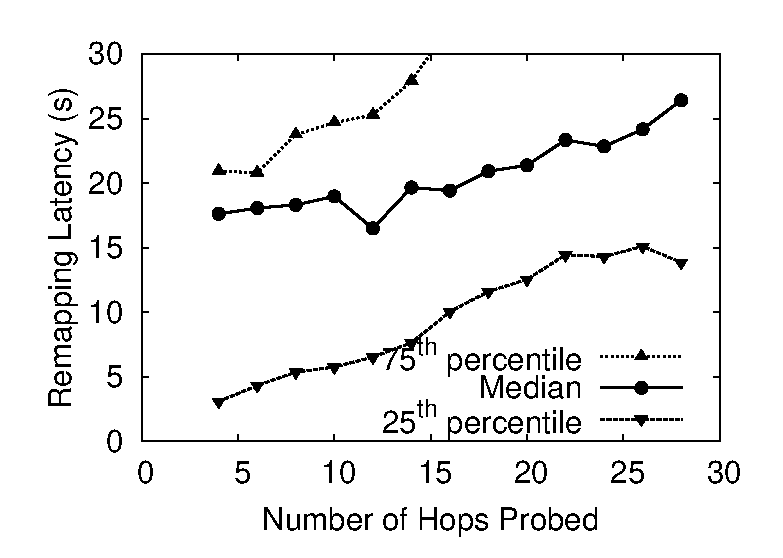
\includegraphics[width=1.05\textwidth]{figs/ptrlatency.eps}
% \caption{Paris traceroute remap latency in the real deployment.}
% \label{fig:deploy.latency.ptr}
% \end{minipage}


To evaluate the prevalence of this problem,
\figstr~\ref{fig:sim.ndisjoint} shows the distribution of the number of
local change zones for consecutive path measurements in our data
set.\footnotemark{}  We observe a single $\LCZ$ in 79\% of cases; here
local remapping, just like complete remapping, will return the correct
new route regardless of detection radius $r'$ (up to statistical errors
in MDA's load balancer discovery).

% , indicating that local remapping will correctly discover the new
% route in most cases.

\footnotetext{We only measure paths when a change is detected, hence all consecutive measurements
observe at least one local change zone.}

Three other factors contribute to minimize the impact of multiple local
change zones.  First, local remapping may remap multiple
$\LCZ$s in one run.  The probability that local remapping will remap 
multiple $\LCZ$s upstream of the detection radius in our data set
is 43\% (in cases where multiple $\LCZ$s exist, not shown).  Second, an
$\LCZ$ which is not remapped when we run local remapping will be
detected and remapped in the future (assuming the new route is stable
enough).  Any $\LCZ$ that is not remapped causes only a temporary
inconsistency.  Third, probing cost savings obtained with local
remapping can be used to increase probing frequency and reduce the
chance that multiple $\LCZ$s appear.

Another limitation of local remapping is that the binary search
mechanism may fail when the relative order of two hops changes between
the previous and current routes.  An extreme, but illustrative, example
is a change from $p_{i-1} = [s, I_1, I_2, I_3, I_4, d]$ to $p_i =
[s, I_4, I_3, I_2, I_1, d]$.  Only 0.9\% of path changes in our data set
reorder hops.  As hop reordering is rare, we take the conservative
approach of remapping the whole path when we detect it. 

Finally, a change may of course occur during remapping.  
This may cause incorrect measurements regardless of remapping approach.  
In practice, \dtrack{} will correct these errors when it reprobes the path, detects that it has
changed, and consequently remaps it.
